\documentclass{article}

% ---- packages and config ---- 
\usepackage[a4paper, vmargin=4cm]{geometry}
\usepackage[bookmarks,hidelinks,pdfusetitle]{hyperref}
\usepackage[T1]{fontenc}
\usepackage{fourier,microtype}
\usepackage[fleqn]{mathtools}
\usepackage{amsthm,amssymb}
\usepackage[table, hyperref, x11names]{xcolor}
\usepackage{enumitem,booktabs,array,tabu,graphicx,tikz}
\usepackage[style=ieee]{biblatex}
\hypersetup{pdfstartview=FitH, pdfpagemode=UseNone, pdfpagelayout=OneColumn, pdfcreator={S Rohit} }
\setcounter{page}{0}
\setlength{\parindent}{0pt}
\linespread{1.35}
\widowpenalty=10000
\clubpenalty=10000
\setlength{\mathindent}{0pt}
\def\[#1\]{\begin{align*}#1\end{align*}}
\colorlet{HighlightColor}{DodgerBlue4}
\colorlet{HyperlinkColor}{HighlightColor!90}
\colorlet{CommentColor}{Azure4}
\setlist{leftmargin=*,itemsep=0pt}
\setlist*[itemize]{label=\textcolor{HighlightColor}{\textbullet}}
\tabulinesep = 4pt
\tabulinestyle{CommentColor!50}
\newcommand{\x}{\mathbf{x}}
\newcommand{\K}{\hat{k}}
\newcommand{\gray}[1]{\textcolor{CommentColor}{#1}}
\newcommand{\Hyperlink}[2]{\href{#1}{\textcolor{HyperlinkColor}{\underline{#2}}}}

% ---- document ---- 
\addbibresource{references.bib}
\begin{document}
	\thispagestyle{empty}

\begin{tikzpicture}
	\linespread{1}
	\node (logo) at (1,0) 
		{
\includegraphics[height=3.5em]{fig/logo.pdf}};
	\node[anchor=east, text width=10cm, align=right] (date) at (\textwidth,-1mm) 
		{November 2020};
	\node[anchor=west, text width=10cm, inner xsep = 2mm] (course) at (logo.east) 
		{{\small IIT-GOA CS-561}\\\textbf{Probability \& Statistics}};
	\node[text width = \textwidth, align=center, anchor=north west, outer ysep=5mm] (title) 
		at ([yshift=-8mm] logo.south west) {\Large\bfseries\scshape Naive Bayes Classifier};
	\draw[line width=0.75pt] (title.north west) -- (title.north east);
	\draw[line width=0.75pt] (title.south west) -- (title.south east);
	\node[text width = \textwidth, align=center, anchor=north, outer sep=5mm] at (title.south)
		{	---\enspace \textbf{Rohit S}\enspace ---\\%
			\texttt{\footnotesize <\,rohit2013107@iitgoa.ac.in\,>}%
		};
\end{tikzpicture}
\vspace{5mm}

\begin{center}
	\textbf{Abstract}
\end{center}
\vspace{-1em}
\qquad The project report discusses the concept and implementation 
of \textit{Na\"ive Bayes Classifier} --- a fast and simple classifier that uses Bayes' theorem 
under the assumption that all features are mutually independent for a given class.
Then, the results of testing one such (Guassian) Na\"ive Bayes Classifier against 
an EMNIST dataset of A--Z handwritten alphabets are presented.\\
Python codes for the above classifier are provided at\enspace \url{https://github.com/s-rohit/naive-bayes}\par\medskip
\textbf{Keywords}: machine learning, data mining, probabilistic classifier, Bayesian network models
\par\vspace{1cm}

\tableofcontents


\clearpage
	\section{Theory}
%================

%--------------------
\subsection{Backgroud}
%--------------------
Our goal is to construct a \textbf{classifier} -- a system that accepts an `object' as input and based on certain `features' of the object, attempts to assign a `label' to it.
To do so, the classifier must first have:
\begin{enumerate}[label={\roman*)}, nosep, topsep=0pt]
	\item A \textit{training dataset} to learn about the different objects, their labels and possible features.
	\item A \textit{prediction algorithm} to predict the label of an unknown object given as input.
\end{enumerate}
Objects having the same label are said to belong to the same ``class'' of objects.\\
Depending on the prediction algorithm used, a wide variety of classifiers have been created.

\paragraph{Probabilistic Classifier} a classifier that gives the probability distribution over all possible labels for a given input. The predicted label for that object is then the label with the highest probability.

\paragraph{Confusion Matrix} a tabular representation of how often the system got `confused' between objects of any two classes (mislabelled one as another). Rows represent the actual label of the object tested  and columns represent the predicted labels (or vice-versa). 
Observe that:
\begin{itemize}[nosep]
	\item Diagonal elements = number of successful predictions for a particular class
	\item Trace of the matrix = total number of successful predictions  
	\item Row-wise (or column-wise) sum = number of times an object of that class was tested
	\item Total sum = total number of tests performed
\end{itemize}


%-----------------------------
\subsection{Bayes Classifier}
%-----------------------------
Bayes Classifier is a probabilistic classifier that uses Bayes' theorem to find the probability 
of an object belonging to a particular class.
That is, given an un-labelled object $\mathbf {x} =(x_{1},\ldots ,x_{n})$ with $n$ features, 
we use Bayes' theorem to find the \textit{posterior} probabaility $\Pr(C_k\mid\x)$ 
of object $\x$ having the label $C_k$

$$ \Pr(C_k \mid \x) = \frac{\Pr(C_k)\ \Pr(\x \mid C_k)}{ \Pr(\x) } $$

\begin{itemize}[itemsep=2mm, topsep=4mm]
	\item Likelihood,
		$\Pr(C_k) = \dfrac
			{\text{\small number of $C_k$-labelled objects}}
			{\text{\small total number of objects}}
		$ in training set \hfill \gray{\small (Discrete Uniform Probability Law)}
	\item  Evidence probability,
		$\displaystyle \Pr(\x) = \sum_k \Pr(C_k)\ \Pr(\x \mid C_k)$ 
		\hfill \gray{\small (Total Probability Theorem)}\\[-5mm]
	\item Prior probability,
		$\displaystyle \Pr(\x \mid C_k) = \prod_{i=1}^{n} \Pr(x_{i} \mid x_{1},\ldots ,x_{i-1},C_{k})$ 
		\hfill \gray{\small (Chain Rule in Probability)}
\end{itemize}
Using this, the predicted label $C_{\K}$ for $\x$ is found by calculating
$\displaystyle
	\K = \underset{k \in \{1 \dots K\}}{\operatorname{argmax}}\ \bigg\{
			\Pr(C_k \mid \x)
		\bigg\}
$\\[3mm]
\paragraph{Note} $\Pr(\x)$ remains the same for a given $\x$. Hence we simpify as:
\[
	\K  &= \underset{k \in \{1 \dots K\}}{\operatorname{argmax}}\ \bigg\{
			\Pr(C_k)\ \Pr(\x \mid C_k)
		\bigg\}\\
		&= \underset{k \in \{1 \dots K\}}{\operatorname{argmax}}\,\left\{
			\Pr(C_k) \prod_{i=1}^{n} \Pr(x_{i} \mid x_{1},\ldots ,x_{i-1},C_{k})
		\right\}
\]
\smallskip

\subsubsection{Na\"ive Bayes Classifier}
%---------------------------------------
Na\"ive Bayes classifier is a Bayes classifier that computes $\K$ with the assumption that all features of $\x$ are mutually independent, conditional on the class $C_k$.\par
Under this assumption: $\displaystyle \Pr(x_{i} \mid x_{1},\ldots ,x_{i-1},C_{k}) = \Pr(x_i \mid C_{k})$\par
Hence, for input $\x = (x_1, \dots, x_n)$ the classifier predicts label $C_{\K}$ where \hfill\ 
$ \boxed{
	\K  = \underset{k \in \{1 \dots K\}}{\operatorname{argmax}}\,\left\{
			\Pr(C_k) \prod_{i=1}^{n} \Pr(x_{i} \mid C_{k})
		\right\} 
}$

\subsubsection{Gaussian Na\"ive Bayes}
%-------------------------------------
In case of continuous data, we assume that the values of features for a class follow Gaussian distribution. Let $\mu_{ki}$ and $\sigma^2_{ki}$ be the mean and variance of the values of the $i$\textsuperscript{th} feature of class $C_k$.\\
Then, we get the probability density \enspace
$\boxed{
	p(x_{i} = v_i \mid C_{k}) = 
		\frac1{\sqrt{2\pi\sigma^2_{ki}}}
		\exp\left\{
			-\frac{(v_i - \mu_{ki})^2}{2\sigma^2_{ki}}
		\right\}
}$\\[2mm]
For a small fixed $\delta$, \enspace 
	$\Pr(x_{i} = v_i \pm \delta \mid C_{k}) \;\; \propto\;\;  p(x_{i} = v \mid C_{k})$
	\section{Implementation}
%=======================

The two boxed equations need to be modified before implementing on them on a computer, because:
\begin{enumerate}%[itemsep=1mm]
	\item The product of the probabilites would be a very small number (especially for large $n$); and such numbers cannot be accurately stored on a computer as floating points. 
	If the calculated probability is very small, it may even get approximated to zero!
	\item A smoothing factor will have to be introduced to improve the classifier's tolerance and also support cases where the observed variance of feature in a class is close to 0.
	\item Operations like \texttt{exp}, \texttt{pow}, \texttt{sqrt}, etc are usually very resource-intensive. If we can minimize the number of operations by simplifying those equations, removing unecessary constant terms, or calculating some values beforehand, then we can speed up the classifier.
\end{enumerate}
Hence, in this section we will modify the boxed equations to get a working equation as follows:

\newcommand{\ArgMax}{{\underset{k \in \{1 \dots K\}}{\operatorname{argmax}}}\,}
\newcommand{\ArgMin}{{\underset{k \in \{1 \dots K\}}{\operatorname{argmin}}}\,}
\newcommand{\G}{\color{CommentColor!80}}
\newcommand{\R}{\normalcolor}
\[
	\K  &= \ArgMax\left\{
				\Pr(C_k) 
				\prod_{i=1}^{n} \Pr(x_{i} \mid C_{k}) 
			\right\}
			&& 
			\text{\gray{Boxed-eqn-1}}\\
		%
		&=  \G	 \ArgMax\left\{
			\R		\log \left[
			\R			\Pr(C_k) 
			\R			\prod_{i=1}^{n} \Pr(x_{i} \mid C_{k}) 
			\R		\right] 
			\G	\right\}
			&& 
			\R 	\log(\cdot) \text{ is a monotonic function}\\
		%
		&=  \G	\ArgMax\left\{
			\R		\log \big[ \Pr(C_k) \big] +
			\R		\sum_{i=1}^{n} \log \big[ \Pr(x_{i} \mid C_{k}) \big]
			\G	\right\}
			&&
			\R 	\text{Simplifying}\\
		%
		&=  \G	\ArgMax\left\{
			\R		\log \left( \frac{N_k}{|D|} \right) +
			\G		\sum_{i=1}^{n} \log \big[ \Pr(x_{i} \mid C_{k}) \big]
			\G	\right\}
			&&
			\R 	\text{Frequency } N_k \text{ in training set } D\\
		%
		&=  \G	\ArgMax\left\{
			\R		\log \big(N_k) - \log\big(|D|\big) +
			\G		\sum_{i=1}^{n} \log \big[ \Pr(x_{i} \mid C_{k}) \big]
			\G	\right\}\\
		%
		&=  \G	\ArgMax\left\{
			\R		\log \big(N_k\big) +
			\G		\sum_{i=1}^{n} \log \big[ \Pr(x_{i} \mid C_{k}) \big]
			\G	\right\}
			&&
			\R 	\text{removing $|D|$ constant}\\
		%
		&=  \G	\ArgMax\left\{
			\G		\log \big(N_k\big) +
			\R		\sum_{i=1}^{n} \log \left[ 
						\frac1{\sqrt{2\pi\sigma^2_{ki}}}
						\exp\left\{
							-\frac{(v_i - \mu_{ki})^2}{2\sigma^2_{ki}}
						\right\}
					\right]
			\G	\right\}
			&&
			\R 	\text{Using boxed-eqn-2}\\
		%
		&=  \G	\ArgMax\left\{
			\G		\log \big(N_k\big)
			\R		- \sum_{i=1}^{n} \left[
						\frac12 \log \big( 2\sigma^2_{ki} \big) + \frac{\log(\pi)}2 +
						\frac{(v_i - \mu_{ki})^2}{2\sigma^2_{ki}}
					\right]
			\G	\right\}
			&&
			\R 	\text{Simplifying}\\
		%
		&=  \G	\ArgMax\left\{
			\R		\log \big(N_k\big)
					- \sum_{i=1}^{n} \left[
						\frac12 \log \big(z_{ki}\big) + 
						\frac{(v_i - \mu_{ki})^2}{z_{ki}}
					\right]
				\right\}
			&&
			\R 	\text{Simplify \& take } z_{ki} = 2\sigma_{ki}^2\\
		%
		&=  \R	\ArgMin\left\{
				\underbrace{
					- \log \big(N_k\big)
					+ \sum_{i=1}^{n} \left[ \frac12 \log \big( z_{ki} \big) \right]
				}_{= m_k, \text{ constant for class }C_k}
					+ \sum_{i=1}^{n} \left[ \frac{(v_i - \mu_{ki})^2}{z_{ki}} \right]
				\right\}
			&&
			 	\text{Reorganizing}
\]

Hence, we get the working formula $\boxed{\K = \ArgMin\left\{
		m_k
		+ \sum_{i=1}^{n} \frac{(v_i - \mu_{ki})^2}{z_{ki}}
	\right\}}$\par\bigskip

Redefine augmented variance $z_{ki} = 2\sigma_{ki}^2 + \xi$ \enspace to include smoothing factor $\xi$\newpage
	\section{Experiment}
%===================

Based on the working formula for $\K$, a Gaussian Na\"ive Bayes classifier was created and tested against 
an EMNIST \Hyperlink{https://drive.google.com/file/d/18ZY7I1ym0E9s2ecqjfvmPSGwlXzsNi2n}{dataset}
of over 370,000 grayscale 28x28 images of A--Z handwritten alphabets.
\begin{itemize}[noitemsep]
	\item Hence, our dataset had 26 classes (A--Z) with 784 features (pixels) each taking one of 256 values.
	\item The entire dataset was randomly divided into testing sets and training sets in 1:9 ratio.
	\item The classifier uses Gaussian distribution model despite the pixels taking discrete values -- because the training set may not have enough samples to plot the distribution of each pixel accurately.
	\item Smoothing factor $\xi \approx 2048$ was found to give the best results. This corresponds to the assumption of a minimum variance of $32^2$ in the values of the features of every class.
\end{itemize}
The results of one such experiment are presented in this section:\\
Python \& C++ codes for the classifier are available at \Hyperlink{https://github.com/s-rohit/naive-bayes}{Github}.

\subsection{Mean and Variance}
%-----------------------------
The mean and variance of the pixels each alphabet are presented as 28x28 grayscale images. \\
As expected, the mean represents ``what that alphabet on average looks like'', and the variance increases towards the edges and the protruding parts of each alphabet.
\begin{figure}[h]
	\centering
	\caption{Mean of pixel values of each alphabet (scaled).}\par
	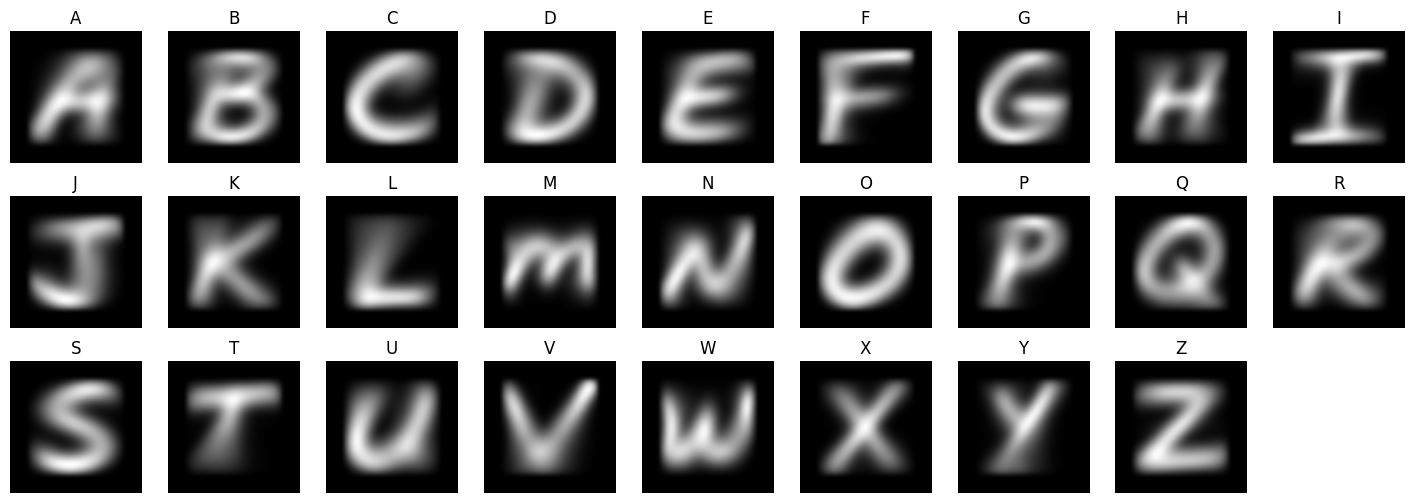
\includegraphics[width=0.725\textwidth]{fig/mean}
	\caption{Variance of pixel values of each alphabet (scaled).}\par
	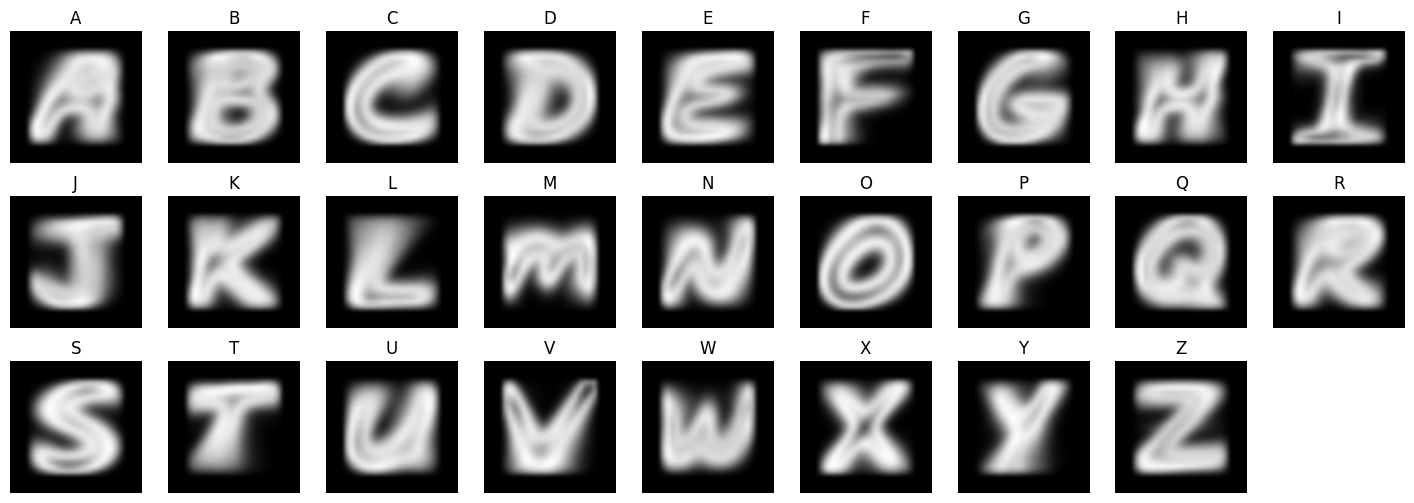
\includegraphics[width=0.725\textwidth]{fig/variance}
\end{figure}

\newpage
\subsection{Confusion matrix and Accuracy}
%----------------------------------------
As described in section 1, the overall and class-wise accuracy are found using the confusion matrix.
\begin{itemize}[nosep]
	\item Overall accuracy = trace of matrix $\div$ total sum
	\item Class-wise accuracy = value$_{ii}$ $\div$ row-wise sum
\end{itemize}
\begin{figure}[h]
	\centering
	\small
	\caption{Accuracy of prediction}\par
	\textbf{Overall accuracy $\approx 70.05\%$}\par\medskip
	\begin{tabu}{|c|c|c |c|c|c |c|c|c |}
		\tabucline-\rowfont\bfseries
		A        &  B      &  C      &  D      &  E      &  F      &  G      &  H      &  I     \\
		74.46\% & 71.78\% & 71.61\% & 69.44\% & 58.81\% & 87.59\% & 78.63\% & 44.46\% & 92.62\% \\ 
		\tabucline-\rowfont\bfseries
		J       &  K      &  L      &  M      &  N      &  O      &  P      &  Q      &  R      \\
		54.55\% & 60.84\% & 73.44\% & 88.69\% & 58.28\% & 82.72\% & 81.42\% & 75.93\% & 45.03\% \\ 
		\tabucline-\rowfont\bfseries
		S       &  T      &  U      &  V      &  W      &  X      &  Y      &  Z      & \\
		66.80\% & 72.14\% & 54.45\% & 88.98\% & 78.62\% & 61.39\% & 78.31\% & 56.03\% & \\
		\tabucline-
	\end{tabu}
	\par\bigskip
	\caption{Confusion matrix}\par
	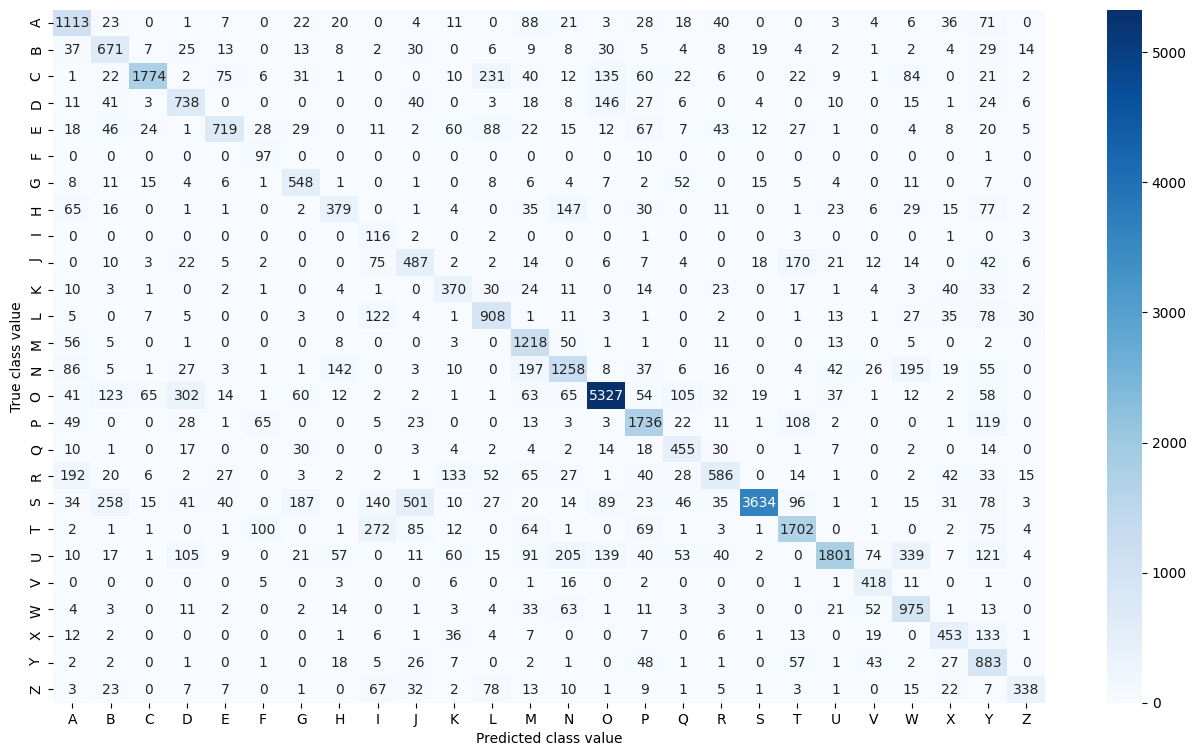
\includegraphics[width=0.99\textwidth, trim={0 0 5cm 0}]{fig/confusion}
\end{figure}

\textbf{Observations}
\begin{itemize}[itemsep=0pt]
	\item Letter `H' has the least accuracy, and is confused for `N' about a third of the time.
	\item Letter `R' has a low accuracy, and is often confused for `A' and `K'.
	\item Letters `F' and `I' seem to have high accuracy, but were not tested as much as others.
	\item Letters `O' and `S' were tested the most; letter `I' has the highest accuracy.
\end{itemize}\newpage
	\section{Conclusion}
%===================

The project provides a basic introduction into the field of machine learning 
and shows a small example of how probability theorems are used in practical applications.
\par\medskip
The Na\"ive Bayes Classifier is fast and easy but the biggest disadvantage is that features are assumed to be independent, which is not true for most real life cases. An improved classifier can be built by removing these (naïve) independence assumptions and using multivariate Gaussian probability distribution.


\addcontentsline{toc}{section}{References}
\nocite{*}
\printbibliography 
\end{document}
